\documentclass[a4paper,12pt]{article}
\usepackage[ngerman]{babel}
\usepackage{multirow}
\usepackage{xltxtra}
\usepackage[utf8x]{inputenc}
\usepackage{fontspec}
\usepackage{eurosym}
\usepackage{graphicx}
\usepackage[paper=a4paper,left=25mm,right=25mm,top=25mm,bottom=25mm]{geometry}
\usepackage{makecell}
\usepackage[table]{xcolor}
\usepackage{float}
\usepackage[normalem]{ulem}
\usepackage{xcolor,colortbl}
\definecolor{Gray}{gray}{0.85}
\usepackage[automark]{scrlayer-scrpage}
\usepackage[
	colorlinks=true,
	urlcolor=blue,
	linkcolor=green
]{hyperref}
\setlength{\parindent}{0em}
\setlength{\parskip}{1ex}
\pagestyle{scrheadings}
\clearscrheadfoot
\begin{document}
\input{theme.tex}
\input{version.tex}
\ohead{Regelstand: \commitDate, id: \commitID}
\title{\tagYear\ Jousting Challenge Regeln}

\makeatletter
\let\inserttitle\@title
\makeatother
\begin{center}
	\rrgerLogo
	\huge                      % Schriftgröße einstellen
	\bfseries                   % Fettdruck einschalten
	\\
	\inserttitle
\end{center}

\begin{center}
Diese Challenge endet mit einem \textbf{einzigen Ausscheidungsturnier}
\\
Die nach Punkten \textbf{8 besten Teams} aller Altersgruppen werden um
Auszeichnungen konkurrieren.
\end{center}
\section{Ziel}
Entwerfe, baue und programmiere einen Linienfolger, der einen Ritter mitführen
kann (leicht gehalten von einem Magneten auf einer Metallplatte), welcher in
einem Lanzenstechen (sog. Tjost) den gegnerischen Ritter nur mithilfe einer
Lanze zu Boden werfen kann.
\section{Wer kann teilnehmen?}
In dieser Challenge kämpfen Teams \textbf{unterschiedlichen Altersgruppen},
üblicherweise:
\begin{itemize}
	\item Altersgruppe ES
	\item Altersgruppe MS
\end{itemize}
\section{Anforderungen}
Autonomer Roboter, basierend auf beliebiger Plattform, der \euro{1.500}  oder
weniger kostet und die folgenden Designbedingungen erfüllt, die beim Check-In
überprüft werden:
\begin{itemize}
	\item Der Roboter kann demonstieren, dass er ein Linienfolgerprogramm
		ausführt indem er der Jousting-Strecke vom Start entlang der
		Kurve bis zur 100 Punkte Linie folgt.
	\item Die Ritterbefestigungsstruktur (Marmeladenglassdeckel) kann mit
		jedem beliebigen Material befestigt werden. Die Art der
		Befestigung darf dem Ritter keine zusätzliche Stütze bieten und
		keine zusätzliche magnetische Haftkraft erzeugen, die dem
		Ritter hilft, an der Struktur befestigt zu bleiben.
	\item Die Ritterbefestigungsstruktur darf sich maximal 10 cm vor dem
		Roboter befinden und maximal eine Höhe von 10 cm über dem Boden
		habe
	\item Der Körper des Ritters ist auf dem erforderlichen Metalldeckel
		völlig freistehend, daher sind KEINE umgebenden Stützsysteme um
		den Metalldeckel herum erlaubt.
	\item Der Ritter ist mit einem rundem Knopfmagneten mit einer Haftkraft
		von 800g an der Metallplatte befestigt.
	\item Es dürfen sich keine weiteren Magneten innerhalb oder außerhalb
		des Ritters oder an der Plattform befinden.
	\item Es muss ein Linienfolgerprogramm mit einem oder mehreren Sensoren
		verwendet werden welches den Roboter führt
	\item Während der eigentlichen Wettbewerbs muss der offizielle Ritter
		des jeweiligen Jahres verwendet werden. Dieser wird am Track
		bereitgestellt. \emph{Dies gilt ebenso für den Marmeladenglasdeckel,
		den Magneten und die Lanze.}
	\item Das Volumen des Roboter darf 65030 cm$^{3}$ \textbf{nicht}
		überschreiten.
\end{itemize}
\section{Allgemeine Spielregeln}
\begin{itemize}
	\item Ein Linienfolgerprogramm muss die Bewegung des Roboters steuern.
	\item Währed der Punktephase gibt es keine festgelegten Gegner, geht
		einfach zu irgendeinem Spielfeld um einen Gegner zu finden
	\item Während eines Duells sind maximal 5 Tjosts erlaubt, eine Tjost
		ist definiert als \textbf{Versuch} beider Roboter den
		gegnerischen Ritter herunterzustoßen.
	\item Wenn alle Tjost genutzt wurden und kein Ritter herunter
		gestoßen wurden, gilt die Tjost als unentschieden. Beide Teams
		überlassen das Spielfeld den wartenden Teams.
	\item Wenn beide Ritter zu Boden fallen, gilt der Ritter, welcher lt.
		Punktrichter zuletzt den Boden berührt als Gewinner.
	\item \textbf{Nur die Lanze} darf den Ritter herunterstoßen. Sollte der
		Ritter durch etwas anderes heruntergestoßen werfen, so wird mit
		der nächsten Tjost fortgefahren (außer es handelt sich um die
		5. Tjost).
	\item \textbf{Nur} die Lanze darf die Mittellinie des Spielfeldes
		überqueren (\textasciitilde13 cm von den jeweiligen 2
		parallelen Linien entfernt).
	\item Die erreichte Punktezahl vermindert sich nach jeder erfolglosen
		Tjost um 10\%. Es gibt maximal 5 Tjosts.
		\emph{Beispiel: Ihr gewinnt die dritte Tjost, Euer Gegner
		landet in der 150, 100 oder 50 Punkte Zone: Eure möglichen
		Punkte wären:}
		\begin{itemize}
			\item $150\cdot0.8 = 120$
			\item $100\cdot0.8 = 80$
			\item $50\cdot0.8 = 40$
		\end{itemize}
	\item Ihr bekommt 10 offiziell gewertete Duelle im Laufe der
		Punktephase dieser Challenge
	\item Die Summe Eurer 5 besten Wertungen wird zur Auswahl zum Turnier
		herangezogen
\end{itemize}
\section{Challenge Spezifikation}
\subsection{Spielfeld}
\includegraphics[width=1\textwidth]{images/track.png}
\begin{itemize}
	\item Zwei parallele ungefähr 2,5 cm breite Linien auf weißer PVC-Plane.
	\item Jede Linie hat zu Beginn eine leichte Kurve.
	\item Ein Meterstab \emph{kann durch die Schiedsrichter} unter der
		Plane entlang der Mittellinie als Schranke (sog. "Tilt")
		platziert werden.
\end{itemize}
\subsection{Punktezonen}
\begin{itemize}
	\item 150 Punkte - 0 cm to 15 cm vom Start
	\item 100 Punkte - 15 cm bis 30 cm vom Start
	\item  50 Punkte - 30 cm bis 90 cm vom Start
\end{itemize}
\begin{center}
	\emph{Alle Abmessungen sind ungefähre Werte}
\end{center}
\section{Punktevergabe}
\begin{itemize}
	\item Die volle Punktzahl wird \textbf{nur} vergeben, wenn ihr euren
		Gegner im \textbf{ersten} von fünf Veruschen herunterstoßt.
		Jeder folgende Versuch verringert die Punkte um 10\%.
		\textbf{Siehe Tabelle unten}.
	\item Höhere Punktezahlen werden erzielt, je näher das Herunterwerfen
		an der Startposition gelingt.
	\item Wenn der Ritter (\emph{nicht die Lanze}) zwischen 2
		Punktebereichen liegt, zählt die höhere Punktezahl.
\end{itemize}
\section{Punktetabelle}
\begin{center}
\begin{tabular}{|c|c|c|c|c|c|c|c|} \hline
	\multicolumn{8}{|c|}{NUR WENN ein Ritter mit der Lanze des Gegners heruntergestoßen wurde}\\
	\multicolumn{8}{|c|}{bekommt der Sieger Punkte}\\
	\multicolumn{8}{|c|}{}\\
	\multicolumn{8}{|c|}{Definition: Tojst - der Versuch beider Roboter den Gegner herunterzustoßen}\\
	\multicolumn{8}{|c|}{}\\
	\multicolumn{8}{|c|}{Jedes Team hat 5 Tjosts um den Gegner herunterzustossen} \\ \hline
	\multicolumn{2}{|c|}{\multirow{2}{*}{\textbf{Punkte pro Tjost}}} & \textbf{1. Tjost} & \textbf{2. Tjost} & \textbf{3. Tjost} & \textbf{4. Tjost} & \textbf{5. Tjost} & 5 Tjosts und \\
	\multicolumn{2}{|c|}{}  & (100\%) & (90\%) & (80\%) & (70\%) & (60\%) & kein Sieger? \\
	\cline{1-7}
	\multirow{3}{*}{\textbf{Punkte}} & 150 Zone & 150 & 135 & 120 & 105 & 90 & Unentschieden: \\
	\cline{2-7}
	& 100 Zone & 100 & 90 & 80 & 70 & 60 & Jedes Team \\
	\cline{2-7}
	& 50  Zone& 50 & 45 & 40 & 35 & 30 & 5 Punkte \\
	\hline
	\multicolumn{8}{|c|}{Der Verlierer bekommt 0 Punkte}\\
	\hline
\end{tabular}
\end{center}
\section{Tunierplan}
\begin{itemize}
        \item Die besten acht Mannschaften werden an der Endrunde teilnehmen.
        \item Die aufsteigenden Teams werden entsprechend ihrer Gesamtpunktzahl in die Turnierliste gesetzt (siehe untenstehende Tabelle).
        \item Der zweite Platz ("`Runner Up"') wird verwendet, um den 3. Platz auf der Grundlage des Ergebnisses der Halbfinalrunde zu bestimmen.
\end{itemize}
\begin{figure}[H]
    \centering
    \def\svgwidth{\columnwidth}
    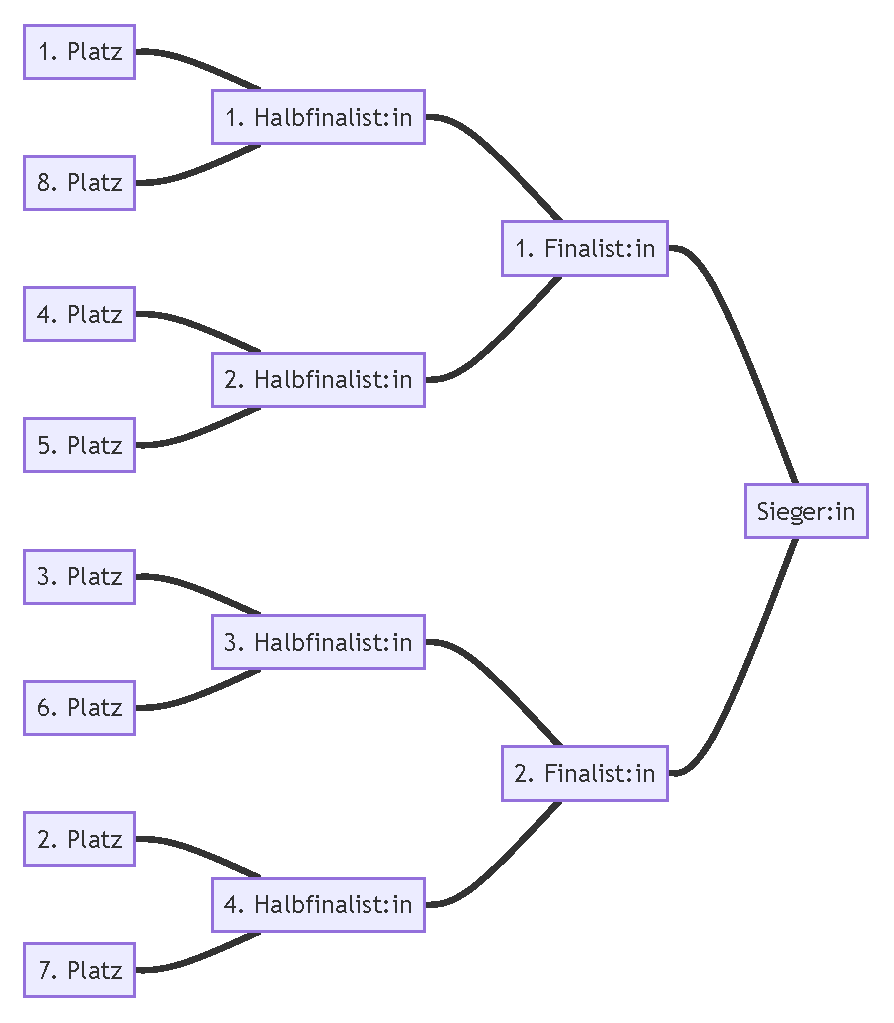
\includegraphics{tournament_score/tournament_score.pdf}
\end{figure}
\end{document}
